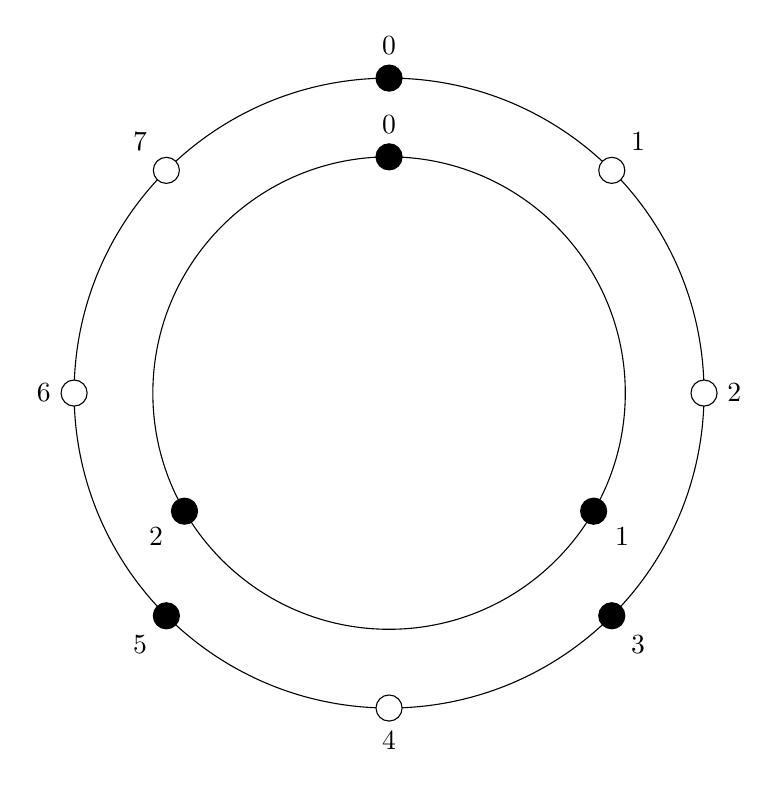
\begin{tikzpicture}[scale=2]
\def \innerradius{1.5}
\node (origin) at (0,0) {};
\draw (origin) circle (\innerradius);
\node (n0) at +(90.0:\innerradius) [circle, draw, fill=black, label = 90.0:0]{};
\node (n1) at +(330.0:\innerradius) [circle, draw, fill=black, label = 330.0:1]{};
\node (n2) at +(210.0:\innerradius) [circle, draw, fill=black, label = 210.0:2]{};
\def \outerradius{2.0}
\node (origin) at (0,0) {};
\draw (origin) circle (\outerradius);
\node (n0) at +(90.0:\outerradius) [circle, draw, fill=black, label = 90.0:0]{};
\node (n1) at +(45.0:\outerradius) [circle, draw, fill=white, label = 45.0:1]{};
\node (n2) at +(0.0:\outerradius) [circle, draw, fill=white, label = 0.0:2]{};
\node (n3) at +(315.0:\outerradius) [circle, draw, fill=black, label = 315.0:3]{};
\node (n4) at +(270.0:\outerradius) [circle, draw, fill=white, label = 270.0:4]{};
\node (n5) at +(225.0:\outerradius) [circle, draw, fill=black, label = 225.0:5]{};
\node (n6) at +(180.0:\outerradius) [circle, draw, fill=white, label = 180.0:6]{};
\node (n7) at +(135.0:\outerradius) [circle, draw, fill=white, label = 135.0:7]{};
\end{tikzpicture}
